\documentclass[utf8x]{beamer}

% This file is a solution template for:

% - Talk at a conference/colloquium.
% - Talk length is about 20min.
% - Style is ornate.

\mode<presentation>
{
  \usetheme{Warsaw}
  % or ...

  %\setbeamercovered{transparent}
  % or whatever (possibly just delete it)
}


\usepackage[english]{babel}
\usepackage{listings}
\usepackage{fancyvrb}
\usepackage{ulem}
\usepackage{color}
\usepackage{alltt}

\usepackage[utf8x]{inputenc}

\input{pygments}

\newcommand\redsout[1]{{\color{red}\sout{\hbox{\color{black}{#1}}}}}
\newcommand{\noop}{}

% or whatever

% Or whatever. Note that the encoding and the font should match. If T1
% does not look nice, try deleting the line with the fontenc.


\title[Runtime Feedback in a Meta-Tracing JIT]{Runtime Feedback in a Meta-Tracing JIT for Efficient Dynamic Languages}

\author[Carl Friedrich Bolz et. al.]{\emph{Carl Friedrich Bolz}\inst{1} \and Antonio Cuni\inst{3} \and Maciej Fijałkowski\inst{2} \and Michael Leuschel\inst{1} \and Samuele Pedroni\inst{3} \and Armin Rigo\inst{1}}
% - Give the names in the same order as the appear in the paper.
% - Use the \inst{?} command only if the authors have different
%   affiliation.

\institute[Heinrich-Heine-Universität Düsseldorf]
{$^1$Heinrich-Heine-Universität Düsseldorf, STUPS Group, Germany \and

 $^2$merlinux GmbH, Hildesheim, Germany \and

 $^3$Open End, Göteborg, Sweden \and
}

\date{ICOOOLPS 2011, July 26, 2011}
% - Either use conference name or its abbreviation.
% - Not really informative to the audience, more for people (including
%   yourself) who are reading the slides online


% If you have a file called "university-logo-filename.xxx", where xxx
% is a graphic format that can be processed by latex or pdflatex,
% resp., then you can add a logo as follows:




% Delete this, if you do not want the table of contents to pop up at
% the beginning of each subsection:
%\AtBeginSubsection[]
%{
%  \begin{frame}<beamer>
%    \frametitle{Outline}
%    \tableofcontents[currentsection,currentsubsection]
%  \end{frame}
%}


% If you wish to uncover everything in a step-wise fashion, uncomment
% the following command: 

%\beamerdefaultoverlayspecification{<+->}


\begin{document}

\begin{frame}
  \titlepage
\end{frame}

\begin{frame}
  \frametitle{Good JIT Compilers for Dynamic Languages are Hard}
  \begin{itemize}
      \item recent languages like Python, Ruby, JS have complex core semantics
      \item many corner cases, even hard to interpret correctly
      \pause
      \item feedback of runtime information to the compiler is necessary
      \item correct exploitation of this information in the compiler
  \end{itemize}
  \pause
  \begin{block}{Problems}
      \begin{enumerate}
          \item implement all corner-cases of semantics correctly
          \item ... and the common cases efficiently
          \item feed back and exploit runtime information
      \end{enumerate}
  \end{block}
\end{frame}

\begin{frame}
  \frametitle{An Interpreter}
  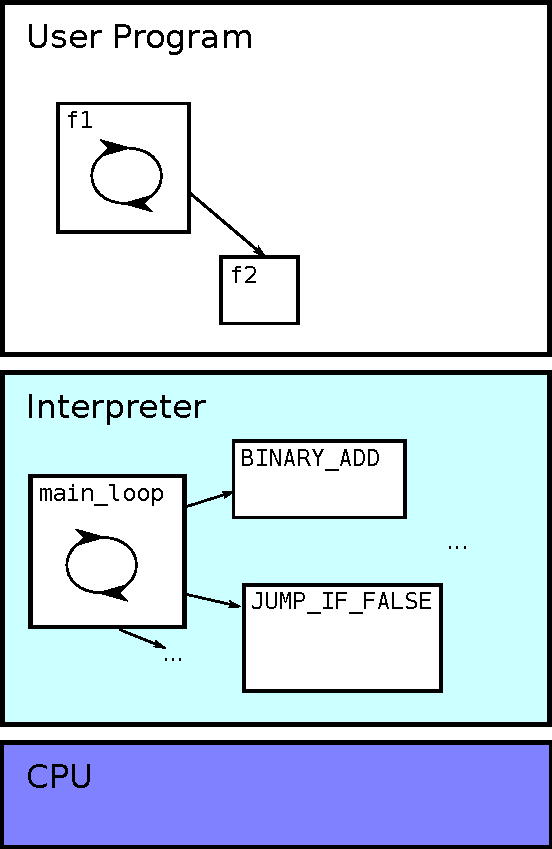
\includegraphics[scale=0.5]{figures/trace01.pdf}
\end{frame}

\begin{frame}
  \frametitle{A Tracing JIT}
  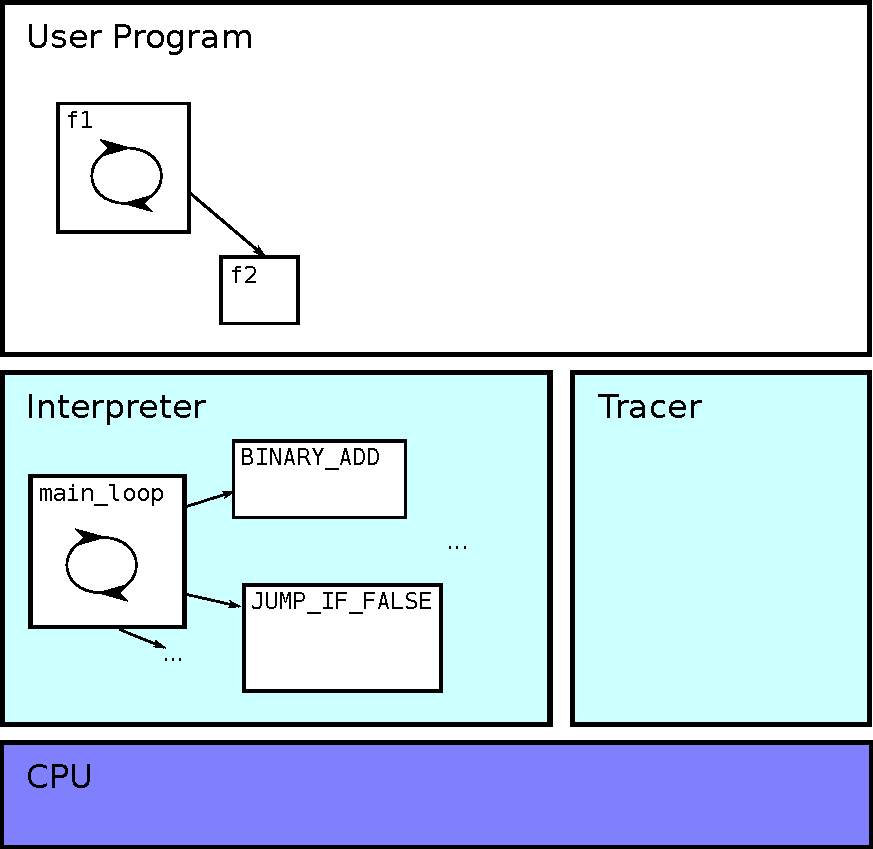
\includegraphics[scale=0.5]{figures/trace02.pdf}
\end{frame}

\begin{frame}
  \frametitle{A Tracing JIT}
  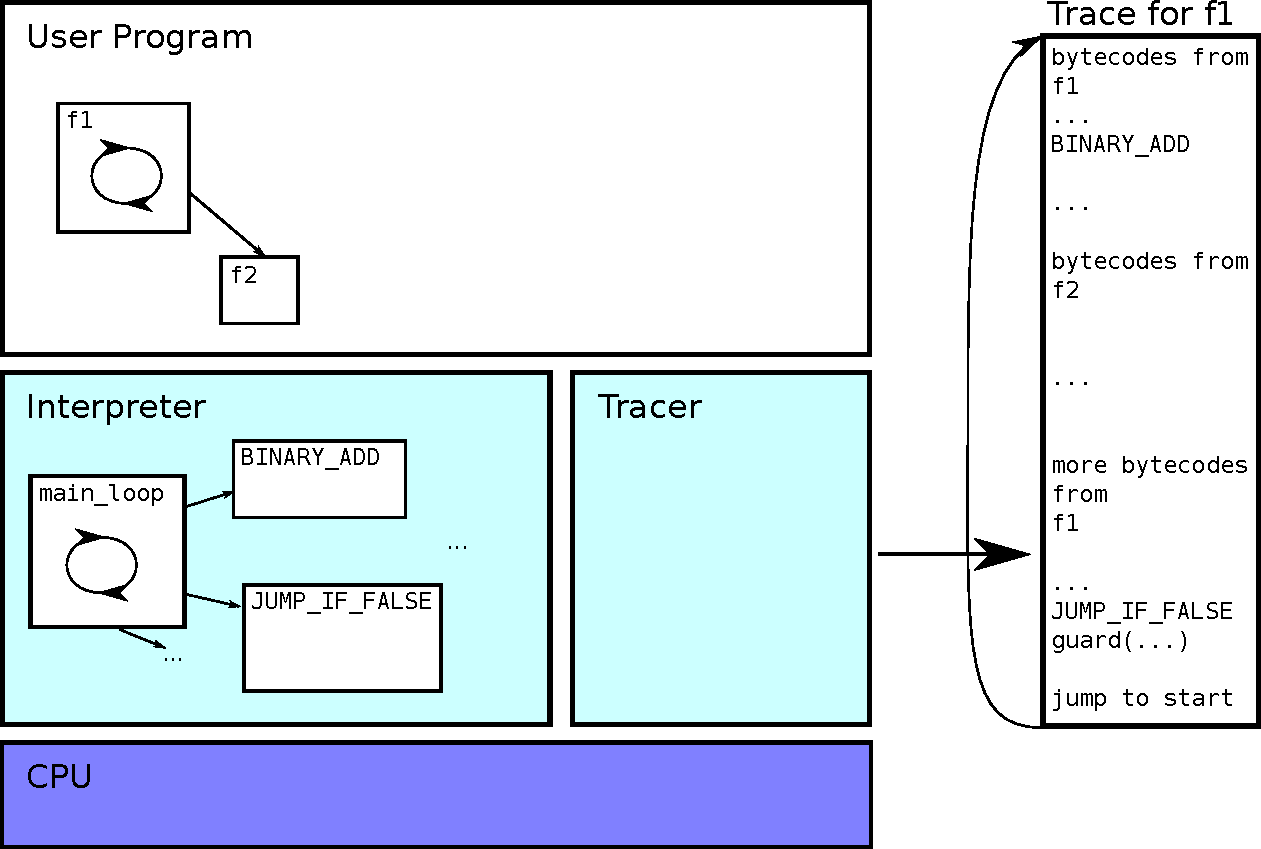
\includegraphics[scale=0.5]{figures/trace03.pdf}
\end{frame}

\begin{frame}
  \frametitle{A Tracing JIT}
  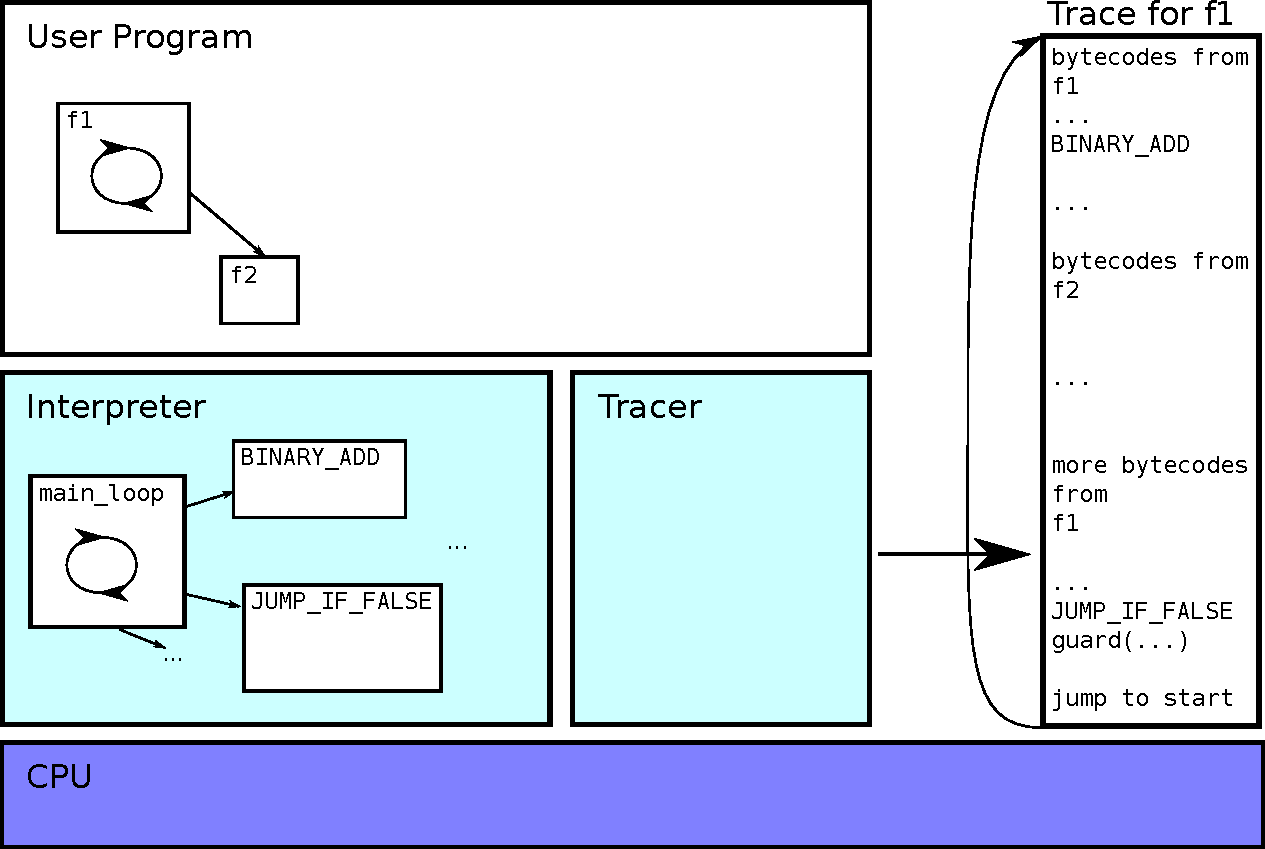
\includegraphics[scale=0.5]{figures/trace04.pdf}
\end{frame}

\begin{frame}
  \frametitle{Tracing JITs}
  Advantages:
  \begin{itemize}
      \item can be added to existing VM
      \item interpreter does a lot of work
      \item can fall back to interpreter for uncommon paths
  \end{itemize}
\end{frame}

\begin{frame}
  \frametitle{Granularity Problems}
  \begin{itemize}
      \item if the tracer records bytecode, not enough information is there
      \item many dynamic languages have bytecodes that contain complex logic
      \item need to expand the bytecode in the trace into something more explicit
      \item this duplicates the lanuage semantics in the tracer/optimizer
  \end{itemize}
\end{frame}

\begin{frame}
  \frametitle{Example: Attribute Reads in Python}
  What happens when an attribute \texttt{x.m} is read? (simplified)
  \pause
  \begin{itemize}
      \item check for \texttt{x.\_\_getattribute\_\_}, if there, call it
      \pause
      \item look for the attribute in the object's dictionary, if it's there, return it
      \pause
      \item walk up the MRO and look in each class' dictionary for the attribute
      \pause
      \item if the attribute is found, call its \texttt{\_\_get\_\_} attribute and return the result
      \pause
      \item if the attribute is not found, look for \texttt{x.\_\_getattr\_\_}, if there, call it
      \pause
      \item raise an \texttt{AttributeError}
  \end{itemize}
  \pause
  all this is one bytecode
\end{frame}

\begin{frame}
  \frametitle{Idea of Meta-Tracing}
  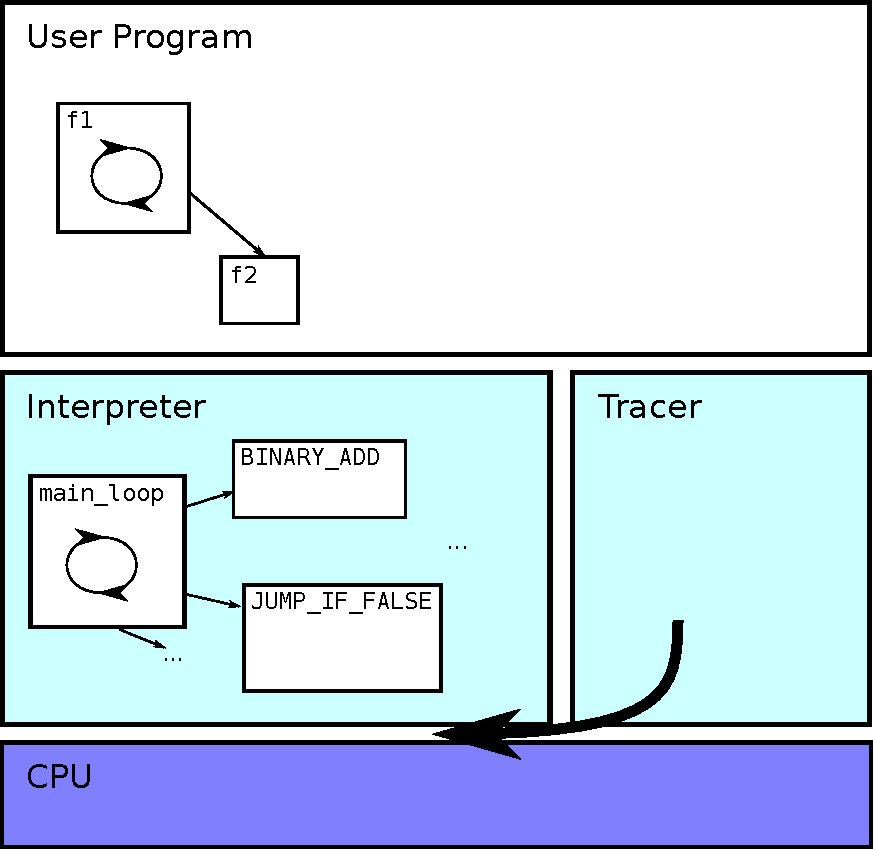
\includegraphics[scale=0.5]{figures/trace05.pdf}
\end{frame}

\begin{frame}
  \frametitle{Meta-Tracing}
  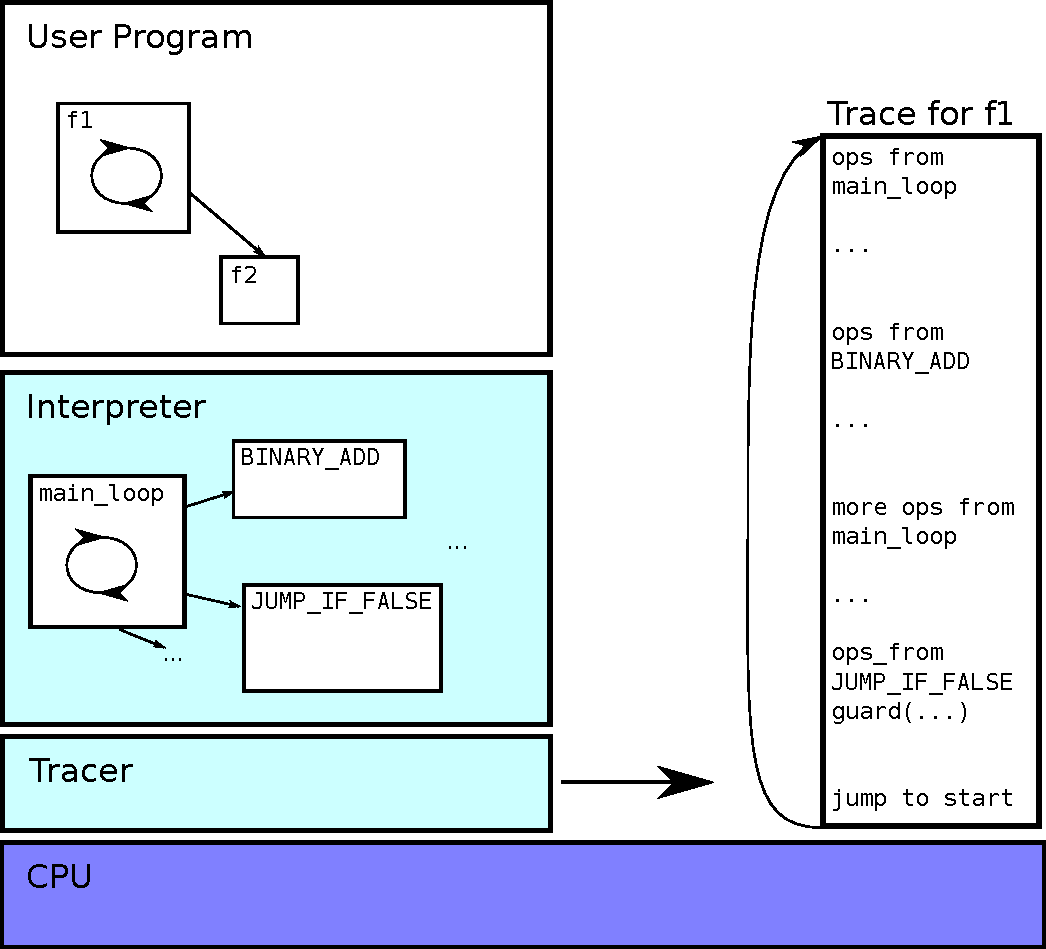
\includegraphics[scale=0.5]{figures/metatrace01.pdf}
\end{frame}

\begin{frame}
  \frametitle{Meta-Tracing JITs}
  \begin{block}{Advantages:}
    \begin{itemize}
        \item semantics are always like that of the interpreter
        \item trace fully contains language semantics
        \item meta-tracers can be reused for various interpreters
    \end{itemize}
  \end{block}
  \pause
  a few meta-tracing systems have been built:
  \begin{itemize}
      \item Sullivan et.al. describe a meta-tracer using the Dynamo RIO system
      \item Yermolovich et.al. run a Lua implementation on top of a tracing JS implementation
      \item SPUR is a tracing JIT for CLR bytecodes, which is used to speed up a JS implementation in C\#
  \end{itemize}
\end{frame}

\begin{frame}
  \frametitle{PyPy}
  A general environment for implementing dynamic languages
  \pause
  \begin{block}{Approach}
      \begin{itemize}
          \item write an interpreter for the language in RPython
          \item compilable to an efficient C-based VM
          \pause
          \item (RPython is a restricted subset of Python)
      \end{itemize}
  \end{block}
  \pause
  \begin{block}{PyPy's Meta-Tracing JIT}
      \begin{itemize}
          \item PyPy contains a meta-tracing JIT for interpreters in RPython
          \item needs a few source-code hints (or annotations) \emph{in the interpreter}
          \item powerful general optimizations
      \end{itemize}
  \end{block}
\end{frame}

\begin{frame}
  \frametitle{Runtime Feedback}
  Problems of Naive Meta-Tracing:
  \begin{itemize}
      \item no runtime feedback of user-level types
      \item tracer does not know about invariants in the interpreter
  \end{itemize}
  \pause
  \begin{block}{Proposed Solutions}
      \begin{itemize}
          \item introduce \textit{hints} that the interpreter-author can use
          \item hints are annotation in the interpreter
          \item they give information to the meta-tracer
          \pause
          \item two hints presented here
          \item one to induce runtime feedback of arbitrary information
          \item the second one to influence constant folding
      \end{itemize}
  \end{block}
\end{frame}


\begin{frame}
  \frametitle{Example: Instances with Maps}
  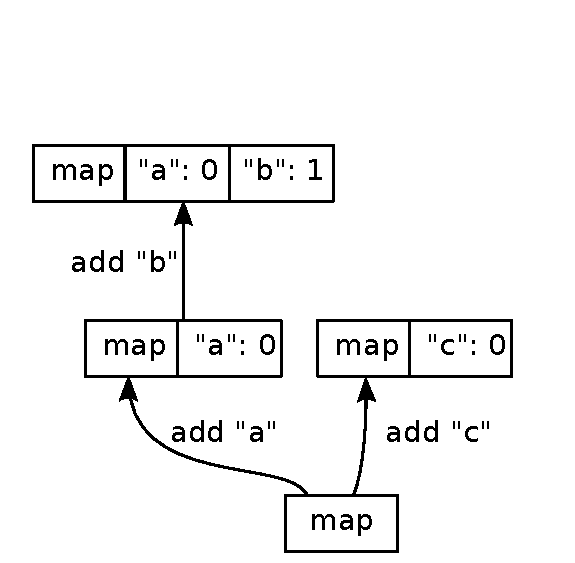
\includegraphics[scale=0.7]{figures/map01.pdf}
\end{frame}

\begin{frame}
  \frametitle{Example: Instances with Maps}
  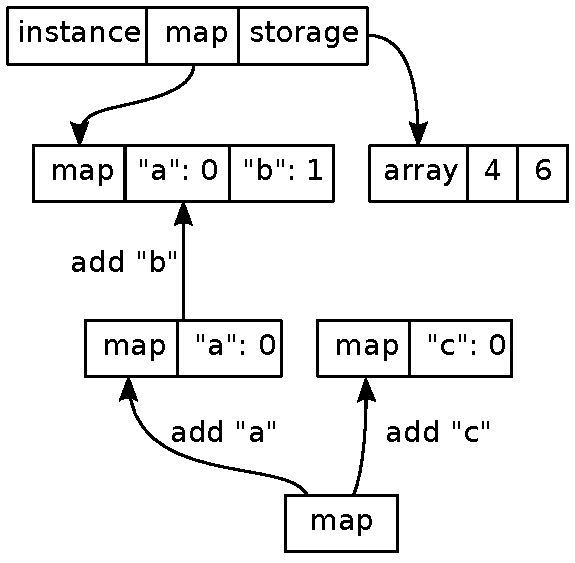
\includegraphics[scale=0.7]{figures/map02.pdf}
\end{frame}

\begin{frame}
  \frametitle{Example: Instances with Maps}
  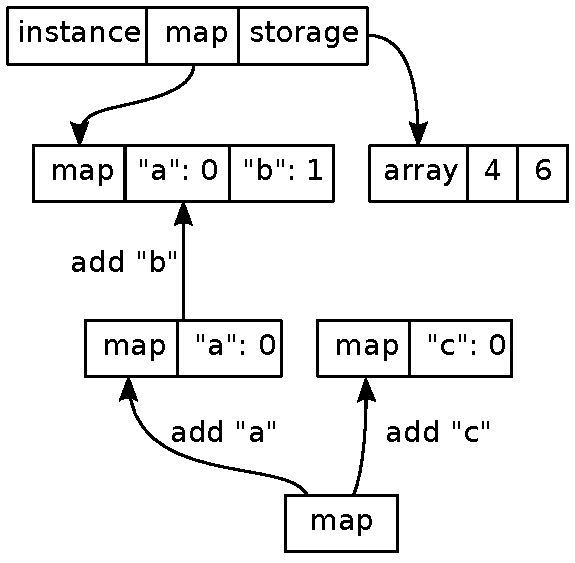
\includegraphics[scale=0.7]{figures/map03.pdf}
\end{frame}

\begin{frame}[containsverbatim]
\frametitle{Map Implementation}

\begin{Verbatim}[commandchars=\\\{\}]
\PY{k}{class} \PY{n+nc}{Map}\PY{p}{(}\PY{n+nb}{object}\PY{p}{)}\PY{p}{:}
    \PY{k}{def} \PY{n+nf}{\PYZus{}\PYZus{}init\PYZus{}\PYZus{}}\PY{p}{(}\PY{n+nb+bp}{self}\PY{p}{,} \PY{n}{indexes}\PY{p}{)}\PY{p}{:}
        \PY{n+nb+bp}{self}\PY{o}{.}\PY{n}{indexes} \PY{o}{=} \PY{n}{indexes}
        \PY{o}{.}\PY{o}{.}\PY{o}{.}

    \PY{k}{def} \PY{n+nf}{getindex}\PY{p}{(}\PY{n+nb+bp}{self}\PY{p}{,} \PY{n}{name}\PY{p}{)}\PY{p}{:}
        \PY{k}{return} \PY{n+nb+bp}{self}\PY{o}{.}\PY{n}{indexes}\PY{o}{.}\PY{n}{get}\PY{p}{(}\PY{n}{name}\PY{p}{,} \PY{o}{-}\PY{l+m+mi}{1}\PY{p}{)}

    \PY{k}{def} \PY{n+nf}{add\PYZus{}attribute}\PY{p}{(}\PY{n+nb+bp}{self}\PY{p}{,} \PY{n}{name}\PY{p}{)}\PY{p}{:}
        \PY{o}{.}\PY{o}{.}\PY{o}{.}

\PY{n}{EMPTY\PYZus{}MAP} \PY{o}{=} \PY{n}{Map}\PY{p}{(}\PY{p}{\PYZob{}}\PY{p}{\PYZcb{}}\PY{p}{)}
\end{Verbatim}
\end{frame}

\begin{frame}[plain,containsverbatim]
\begin{Verbatim}[commandchars=\\\{\}]
\PY{k}{class} \PY{n+nc}{Instance}\PY{p}{(}\PY{n+nb}{object}\PY{p}{)}\PY{p}{:}
    \PY{k}{def} \PY{n+nf}{\PYZus{}\PYZus{}init\PYZus{}\PYZus{}}\PY{p}{(}\PY{n+nb+bp}{self}\PY{p}{)}\PY{p}{:}
        \PY{n+nb+bp}{self}\PY{o}{.}\PY{n}{map} \PY{o}{=} \PY{n}{EMPTY\PYZus{}MAP}
        \PY{n+nb+bp}{self}\PY{o}{.}\PY{n}{storage} \PY{o}{=} \PY{p}{[}\PY{p}{]}

    \PY{k}{def} \PY{n+nf}{getfield}\PY{p}{(}\PY{n+nb+bp}{self}\PY{p}{,} \PY{n}{name}\PY{p}{)}\PY{p}{:}
        \PY{n}{index} \PY{o}{=} \PY{n+nb+bp}{self}\PY{o}{.}\PY{n}{map}\PY{o}{.}\PY{n}{getindex}\PY{p}{(}\PY{n}{name}\PY{p}{)}
        \PY{k}{if} \PY{n}{index} \PY{o}{!=} \PY{o}{-}\PY{l+m+mi}{1}\PY{p}{:}
            \PY{k}{return} \PY{n+nb+bp}{self}\PY{o}{.}\PY{n}{storage}\PY{p}{[}\PY{n}{index}\PY{p}{]}
        \PY{k}{return} \PY{n+nb+bp}{None}

    \PY{k}{def} \PY{n+nf}{write\PYZus{}attribute}\PY{p}{(}\PY{n+nb+bp}{self}\PY{p}{,} \PY{n}{name}\PY{p}{,} \PY{n}{value}\PY{p}{)}\PY{p}{:}
        \PY{o}{.}\PY{o}{.}\PY{o}{.}
\end{Verbatim}
\end{frame}

\begin{frame}[plain,containsverbatim]
\frametitle{Trace for Code \texttt{inst.a + inst.b}}
\begin{lstlisting}[mathescape,escapechar=|,basicstyle=\ttfamily]]
# $inst_1$.getfield("a")
$map_1$ = $inst_1$.map
$index_1$ = Map.getindex($map_1$, "a")
guard($index_1$ != -1)
$storage_1$ = $inst_1$.storage
$result_1$ = $storage_1$[$index_1$]
|\pause|
# $inst_1$.getfield("b")
$map_2$ = $inst_1$.map
$index_2$ = Map.getindex($map_2$, "b")
guard($index_2$ != -1)
$storage_2$ = $inst_1$.storage
$result_2$ = $storage_2$[$index_2$]

$v_1$ = $result_1$ + $result_2$
\end{lstlisting}
\end{frame}

\begin{frame}[plain,containsverbatim]
\frametitle{Trace for Code \texttt{inst.a + inst.b}}
\begin{lstlisting}[mathescape,escapechar=|,basicstyle=\ttfamily]]
# $inst_1$.getfield("a")
$map_1$ = $inst_1$.map
$index_1$ = Map.getindex($map_1$, "a")
guard($index_1$ != -1)
$storage_1$ = $inst_1$.storage
$result_1$ = $storage_1$[$index_1$]

# $inst_1$.getfield("b")
$map_2$ = $inst_1$.map
$index_2$ = Map.getindex($map_2$, "b")
guard($index_2$ != -1)
$storage_2$ = $inst_1$.storage
$result_2$ = $storage_2$[$index_2$]

$v_1$ = $result_1$ + $result_2$
\end{lstlisting}
\end{frame}

\begin{frame}[containsverbatim]
  \frametitle{Runtime Feedback Controlled by the Interpreter Author}
  \begin{itemize}
      \item give the interpreter author a way to feed back runtime values into the trace
      \item written as \texttt{promote(x)}
      \item captures the argument's runtime value during tracing
      \item should be used only for variables that take few values
  \end{itemize}
  \pause
\end{frame}

\begin{frame}[containsverbatim]
  \frametitle{Tiny Example}
  \begin{minipage}[b]{6cm}
      \centering
      {\noop
      \begin{lstlisting}[mathescape,basicstyle=\ttfamily]
def f1(x, y):
    promote(x)
    z = x * 2 + 1
    return z + y
      \end{lstlisting}
      }
  \end{minipage}
  \vline
  \hspace{0.5cm}
  \begin{minipage}[b]{4cm}
      {\noop
      \begin{lstlisting}[mathescape,escapechar=|,basicstyle=\ttfamily]
guard($x_1$ == 4)
|{\color{gray}$v_1$ = $x_1$ * 2}|
|{\color{gray}$z_1$ = $v_1$ + 1}|
$v_2$ = $z_1$ + $y_1$
return($v_2$)
      \end{lstlisting}
      }
  \end{minipage}
\end{frame}

\begin{frame}
  \frametitle{Foldable Operations Defined by the Interpreter Author}
  \begin{itemize}
      \item let the interpreter author define foldable functions
      \item those functions typically don't look foldable
      \item otherwise there is no need for an annotation
      \item done via a function decorator \texttt{@elidable}
      \pause
      \item decorated functions should be pure
      \item or have idempotent side effects (such as a function that memoizes)
      \item trace optimizer will remove calls to such functions with constant arguments
  \end{itemize}
\end{frame}

\begin{frame}[containsverbatim]
\frametitle{Adding Hints to Maps}

\begin{Verbatim}[commandchars=\\\{\}]
\PY{k}{class} \PY{n+nc}{Map}\PY{p}{(}\PY{n+nb}{object}\PY{p}{)}\PY{p}{:}
    \PY{k}{def} \PY{n+nf}{\PYZus{}\PYZus{}init\PYZus{}\PYZus{}}\PY{p}{(}\PY{n+nb+bp}{self}\PY{p}{,} \PY{n}{indexes}\PY{p}{)}\PY{p}{:}
        \PY{n+nb+bp}{self}\PY{o}{.}\PY{n}{indexes} \PY{o}{=} \PY{n}{indexes}
        \PY{o}{.}\PY{o}{.}\PY{o}{.}

    \PY{n+nd}{@elidable}
    \PY{k}{def} \PY{n+nf}{getindex}\PY{p}{(}\PY{n+nb+bp}{self}\PY{p}{,} \PY{n}{name}\PY{p}{)}\PY{p}{:}
        \PY{k}{return} \PY{n+nb+bp}{self}\PY{o}{.}\PY{n}{indexes}\PY{o}{.}\PY{n}{get}\PY{p}{(}\PY{n}{name}\PY{p}{,} \PY{o}{-}\PY{l+m+mi}{1}\PY{p}{)}

    \PY{k}{def} \PY{n+nf}{add\PYZus{}attribute}\PY{p}{(}\PY{n+nb+bp}{self}\PY{p}{,} \PY{n}{name}\PY{p}{)}\PY{p}{:}
        \PY{o}{.}\PY{o}{.}\PY{o}{.}

\PY{n}{EMPTY\PYZus{}MAP} \PY{o}{=} \PY{n}{Map}\PY{p}{(}\PY{p}{\PYZob{}}\PY{p}{\PYZcb{}}\PY{p}{)}
\end{Verbatim}
\end{frame}

\begin{frame}[containsverbatim]
\frametitle{Adding Hints to Maps}

\begin{Verbatim}[commandchars=\\\{\}]
\PY{k}{class} \PY{n+nc}{Instance}\PY{p}{(}\PY{n+nb}{object}\PY{p}{)}\PY{p}{:}
    \PY{k}{def} \PY{n+nf}{\PYZus{}\PYZus{}init\PYZus{}\PYZus{}}\PY{p}{(}\PY{n+nb+bp}{self}\PY{p}{)}\PY{p}{:}
        \PY{n+nb+bp}{self}\PY{o}{.}\PY{n}{map} \PY{o}{=} \PY{n}{EMPTY\PYZus{}MAP}
        \PY{n+nb+bp}{self}\PY{o}{.}\PY{n}{storage} \PY{o}{=} \PY{p}{[}\PY{p}{]}

    \PY{k}{def} \PY{n+nf}{getfield}\PY{p}{(}\PY{n+nb+bp}{self}\PY{p}{,} \PY{n}{name}\PY{p}{)}\PY{p}{:}
        \PY{n}{promote}\PY{p}{(}\PY{n+nb+bp}{self}\PY{o}{.}\PY{n}{map}\PY{p}{)}
        \PY{n}{index} \PY{o}{=} \PY{n+nb+bp}{self}\PY{o}{.}\PY{n}{map}\PY{o}{.}\PY{n}{getindex}\PY{p}{(}\PY{n}{name}\PY{p}{)}
        \PY{k}{if} \PY{n}{index} \PY{o}{!=} \PY{o}{-}\PY{l+m+mi}{1}\PY{p}{:}
            \PY{k}{return} \PY{n+nb+bp}{self}\PY{o}{.}\PY{n}{storage}\PY{p}{[}\PY{n}{index}\PY{p}{]}
        \PY{k}{return} \PY{n+nb+bp}{None}

    \PY{k}{def} \PY{n+nf}{write\PYZus{}attribute}\PY{p}{(}\PY{n+nb+bp}{self}\PY{p}{,} \PY{n}{name}\PY{p}{,} \PY{n}{value}\PY{p}{)}\PY{p}{:}
        \PY{o}{.}\PY{o}{.}\PY{o}{.}
\end{Verbatim}
\end{frame}


\begin{frame}[containsverbatim,plain]
  \frametitle{Trace with Hints for Code \texttt{inst.a + inst.b}}
\begin{lstlisting}[mathescape,escapechar=|,basicstyle=\ttfamily]]
# $inst_1$.getfield("a")
$map_1$ = $inst_1$.map
guard($map_1$ == 0xb74af4a8)
|{\color{gray}$index_1$ = Map.getindex($map_1$, "a")}|
|{\color{gray}guard($index_1$ != -1)}|
$storage_1$ = $inst_1$.storage
$result_1$ = $storage_1$[$index_1$]

# $inst_1$.getfield("b")
|{\color{gray}$map_2$ = $inst_1$.map|
|{\color{gray}guard($map_2$ == 0xb74af4a8)}|
|{\color{gray}$index_2$ = Map.getindex($map_2$, "b")}|
|{\color{gray}guard($index_2$ != -1)}|
|{\color{gray}$storage_2$ = $inst_1$.storage}|
$result_2$ = $storage_2$[$index_2$]

$v_1$ = $result_1$ + $result_2$
\end{lstlisting}
\end{frame}

\begin{frame}[containsverbatim,plain]
  \frametitle{Final Trace}
\begin{lstlisting}[mathescape,escapechar=|,basicstyle=\ttfamily]]
$map_1$ = $inst_1$.map
guard($map_1$ == 0xb74af4a8)
$storage_1$ = $inst_1$.storage
$result_1$ = $storage_1$[$0$]
$result_2$ = $storage_2$[$1$]
$v_1$ = $result_1$ + $result_2$
\end{lstlisting}
\end{frame}


\begin{frame}
  \frametitle{Uses of These Hints}
  \begin{block}{\texttt{promote} lets one specialize on various things:}
      \begin{itemize}
          \item user-level types
          \item shapes of instances
          \item the current state of a classes' methods
          \item ...
      \end{itemize}
  \end{block}
  \pause
  \begin{block}{uses of \texttt{@elidable}}
      \begin{itemize}
          \item define immutable fields by decorating a getter
          \item declare arbitrary invariants
      \end{itemize}
      
  \end{block}
\end{frame}

\begin{frame}
  \frametitle{Some Benchmarks}
  \begin{itemize}
      \item benchmarks done using PyPy's Python interpreter
      \item about 30'000 lines of code
      \item 20 calls to \texttt{promote}
      \item 10 applications of \texttt{@elidable}
  \end{itemize}
\end{frame}

\begin{frame}
  \frametitle{Some Benchmarks}
  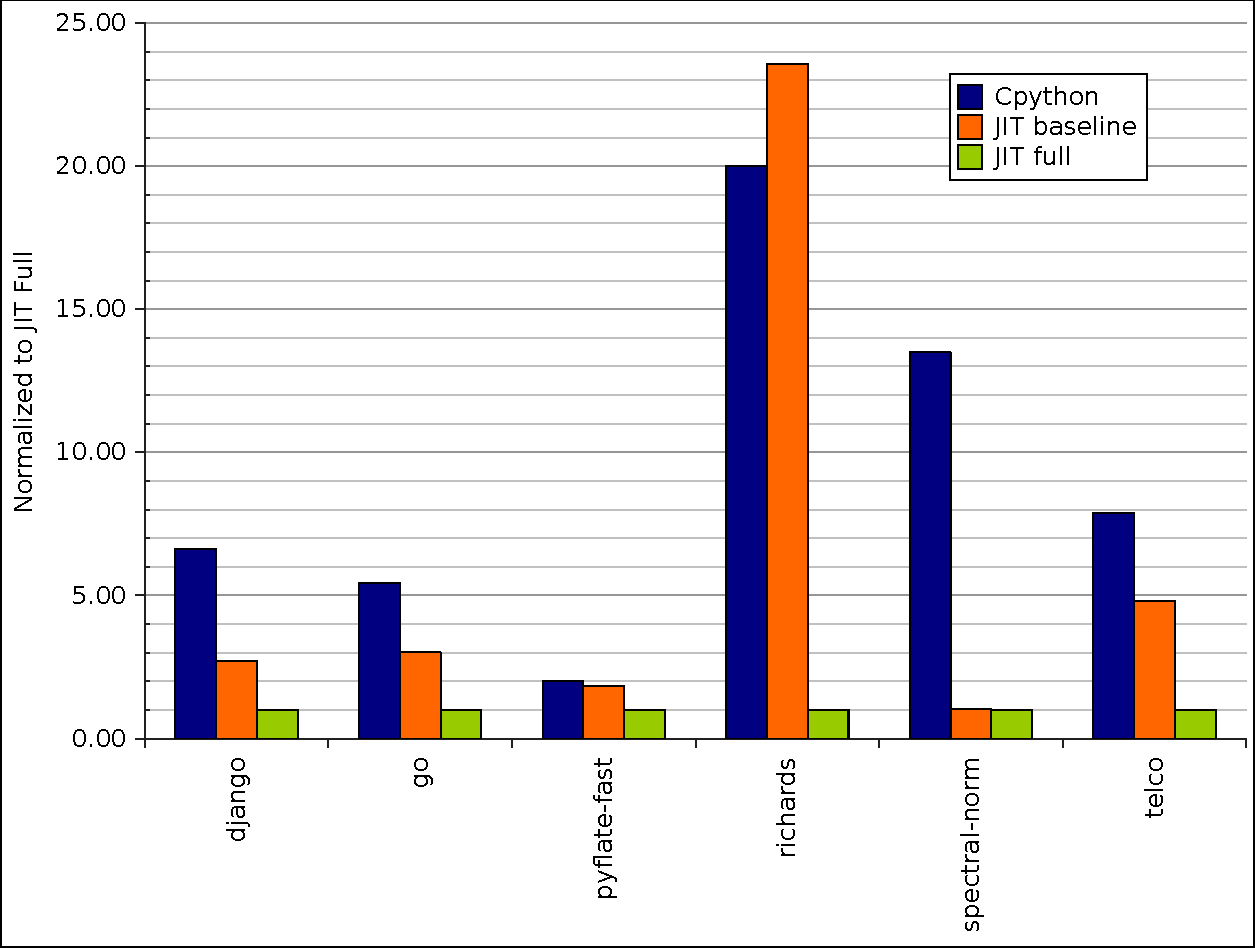
\includegraphics[scale=0.5]{figures/bench.pdf}
\end{frame}

\begin{frame}
  \frametitle{Conclusion}
  \begin{itemize}
      \item meta-tracing can make the efficient implementation of complex dynamic languages easier
      \item only requires to write a correct interpreter
      \item two kinds of hints to be added by the interpreter author allow arbitrary runtime feedback and its exploitation
      \item the hints are expressive enough to re-implement classical optimizations such as maps
      \item usage of the hints leads to good speedups for object-oriented code in PyPy's Python interpreter
  \end{itemize}
\end{frame}

\begin{frame}
  \frametitle{Bonus: Comparison with Partial Evaluation}
  \begin{itemize}
      \pause
      \item the only difference between meta-tracing and partial evaluation is that meta-tracing works
      \pause
      \item ... mostly kidding
      \pause
      \item very similar from the motivation and ideas
      \item PE was never scaled up to perform well on large interpreters
      \item classical PE mostly ahead of time
      \item PE tried very carefully to select the right paths to inline and optimize
      \item quite often this fails and inlines too much or too little
      \item tracing is much more pragmatic: simply look what happens
  \end{itemize}
\end{frame}


\end{document}
